\documentclass[border=4pt]{standalone}
\usepackage{tikz}
\usetikzlibrary{arrows,positioning}
\begin{document}
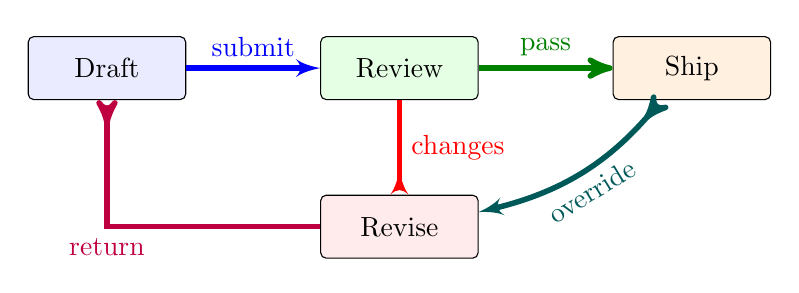
\begin{tikzpicture}[
  node distance=1.2cm and 1.7cm,
  stage/.style={draw,rounded corners=2pt,minimum width=2cm,minimum height=8mm,align=center}
]
  \node[stage,fill=blue!8] (draft) {Draft};
  \node[stage,fill=green!10,right=of draft] (review) {Review};
  \node[stage,fill=orange!12,right=of review] (ship) {Ship};
  \node[stage,fill=red!8,below=of review] (revise) {Revise};

  \draw[blue,line width=2pt,-{latex'}] (draft) -- node[above]{submit} (review);
  \draw[green!50!black,line width=2pt,-{stealth'}] (review) -- node[above]{pass} (ship);
  \draw[red,line width=2pt,-{latex' reversed}] (review) -- node[right]{changes} (revise);
  \draw[purple,line width=2pt,-{stealth' reversed}] (revise) -| node[below]{return} (draft);
  \draw[teal!70!black,line width=2pt,{latex'}-{stealth' reversed}]
    (revise) to[bend right=18] node[below,sloped]{override} (ship);
\end{tikzpicture}
\end{document}
